
\chapter{Priprema podataka} % Main chapter title

\label{Priprema_podataka} % For referencing 

\section{Objedinjavanje CAFA3 i novije \swissprot verzije}

Iz CAFA3 trening skupa izdvojeni su svi validni proteini ( dužine barem 9 i
azbukom od 20 standardnih aminokiselina). U ovom koraku ne izbacujemo proteine
kraće od 40 AK.

Informacije o \swissprot bazi podataka dobijene su iz verzije 2017\_12, iz datoteke
\file{uniprot\_sprot-only2017\_12.tar.gz} \cite{sprot}.
Navedena verzija sadrži 556 196 proteina. 

Od 66 599 validnih CAFA3 proteina 66 530 ima nepromenjen \keyword{primarni
identifikator}. Međutim, 69 slogova u \swissprot bazi sadrže nedostajuće CAFA3
identifikatore kao sekundarne kao što je navedeno u Potpoglavlju
\ref{svis-prot}. Ovo je posledica dva moguća mehanizma:

\begin{enumerate}
  \item Unifikacija nekoliko CAFA3 proteina pod novi slog.
    Rezultat unifikacije prikazan je na Slici \ref{fig:unifikacija_slogova}. Analizom
    ovih promena uspešno su rekonstruisana svega četri nova \swissprot sloga
    koja odgovaraju nedostajućim CAFA3 proteinima. Kako je četri
    suviše mali broj, zbog jednostavnosti nismo ih ubrajali u dalju analizu
    te koristimo samo 66 530 originalnih CAFA3 proteina.

  \begin{figure}[th]
  \centering
  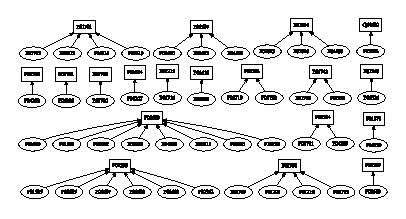
\includegraphics[scale=2]{plots/unifikacija_slogova2.eps}
  \decoRule
  \caption{Unifikacija starih(elipse) na nove slogove u \swissprot bazi podataka}
  \label{fig:unifikacija_slogova}
  \end{figure}

  \item Specijalizacija jednog CAFA3 proteina u više različitih slogova.  Zbog moguće
    statističke redundantnosti ovi slogovi su zanemareni.
\end{enumerate}


Validini CAFA3 proteini anotirani su sa  5 957 različitih GO termina Molekulske
Funkcije (MF) od kojih je 50 zastarelo i izbačeno iz \file{go.obo} datoteke.  U
\swissprot bazi podataka nismo bili u mogućnosti da proverimo samo za MF, ali
ukupno
je izbačeno 319 GO termina.
CAFA3 sadrži 67 MF koje se ne javljaju u \swissprot anotacijama dok
\swissprot sadrži 888 MF koje se ne javljaju u CAFA3 anotacijama.
Pošto \swissprot treba da sadrži svežije (tačnije) informacije, CAFA3 verzija
anotacija je zanemarena u korist novijih \swissprot anotacija. Ove informacije
sumirane su  Tabelom \ref{tab:godiff}

Dodatno, \swissprot sadrži 194 proteina čije se sekvence razlikuje u
odnosu na CAFA3 verziju proteina. Odlučili smo da zadržimo originalne CAFA3
sekvence.

\begin{table}[htpb]
\begin{tabular}{|r|c|c|}
  \hline
                  & CAFA3 & \swissprot       \\
  \hline
  MF termini      & 5 957 &    -    \\
  fali u obo.go   & 60 MF & 319 MF, CC i BP \\
  MF, samo u   & 67    & 888             \\
  \hline
\end{tabular}
  \centering
  \caption{Razlike u GO terminima između CAFA3 i \swissprot}
  \label{tab:godiff}
\end{table}

\section{Grupisanje proteina po GO terminima}

Ako je GO termin A potomak GO termina B tj. važi A \textit{is\_a} B i  želimo da diskutujemo o funkciji B,
onda i svi proteini koji imaju funkciju A (i time pripadaju skupu S\_A) treba da budu sadrzani i u skupu S\_B.
Primetili smo da anotacije ključnih reči ovo već podrazumevaju dok za GO to nije slučaj.
Tek nakon ovakvog grupisanja validno je odbaciti termine koji
anotiraju manje od 20 proteina.  Za predloženo grupisanje koristili smo
algoritam topološkog sortiranja.  Ovom metodom dobijeno je 1781\footnote{Bez
ovog grupisanja imali bi samo 1146 MF termina  koji zadovoljavaju limit od min. 20 proteina} MF termin (od ukupno 11 135 validnih MF termina) sa minimum 20
pridruženih proteina. Ovo uključuje i koreni\footnote{koreni termin ili
koreni čvor ontologije tj.  termin molekulska funkcija} termin . U ovom
koraku uračunati su samo proteini minimalne dužine 40 AK.

% \section{Ontologije gena i ključne reči}
\section{Mapiranje između GO termina i \swissprot ključnih reči}

U nastavku razmatramo samo ključne reči kategorije MF
i načine na koje ih možemo povezati sa ekvivalentnim MF terminima.
Direktno mapiranje sa \keyword{ključnih reči} na GO
termine nije uvek moguće.  Neke ključne reči (\textit{Represor, Cyclin, Activator,
Superantigen, Tumorantigen...}) nemaju odgovarajući GO termin. Od 226 ključnih
reči svega 175 ima odgovarajući GO termin, od kojih 175 ključnih reči
postoji 105 mapiranja na MF termin, 59 na BP
i 11 na CC.  Dakle, za 70 MF ključnih reči ne postoji direktno mapiranje na MF
termine.

Slika \ref{fig:KWtop20dis} prikazuje moguća direktna mapiranja
(dobijena iz \file{keywords.txt}) za 20 neuređenih MF ključnih reči pronađenih
u radu \parencite{Xie2007}.  U našoj verziji \file{keywords.txt} Antigen je
izbačen i zamenjen specijalizovanijom podelom. Tri ključne reči nemaju
mapiranje, dve se mapiraju na ćelijske komponente, osam na biološke procese i
svega šest na molekulske funkcije. Statistički značajne ključne reči su
ljubičaste dok radi kompletnosti navodimo neke njihove specijalizacije i
generalizacije koje su obojene sivo. GO termini su predstavljeni manjim
kružićima. 

\begin{figure}[th]
\hspace*{-2.2cm} 
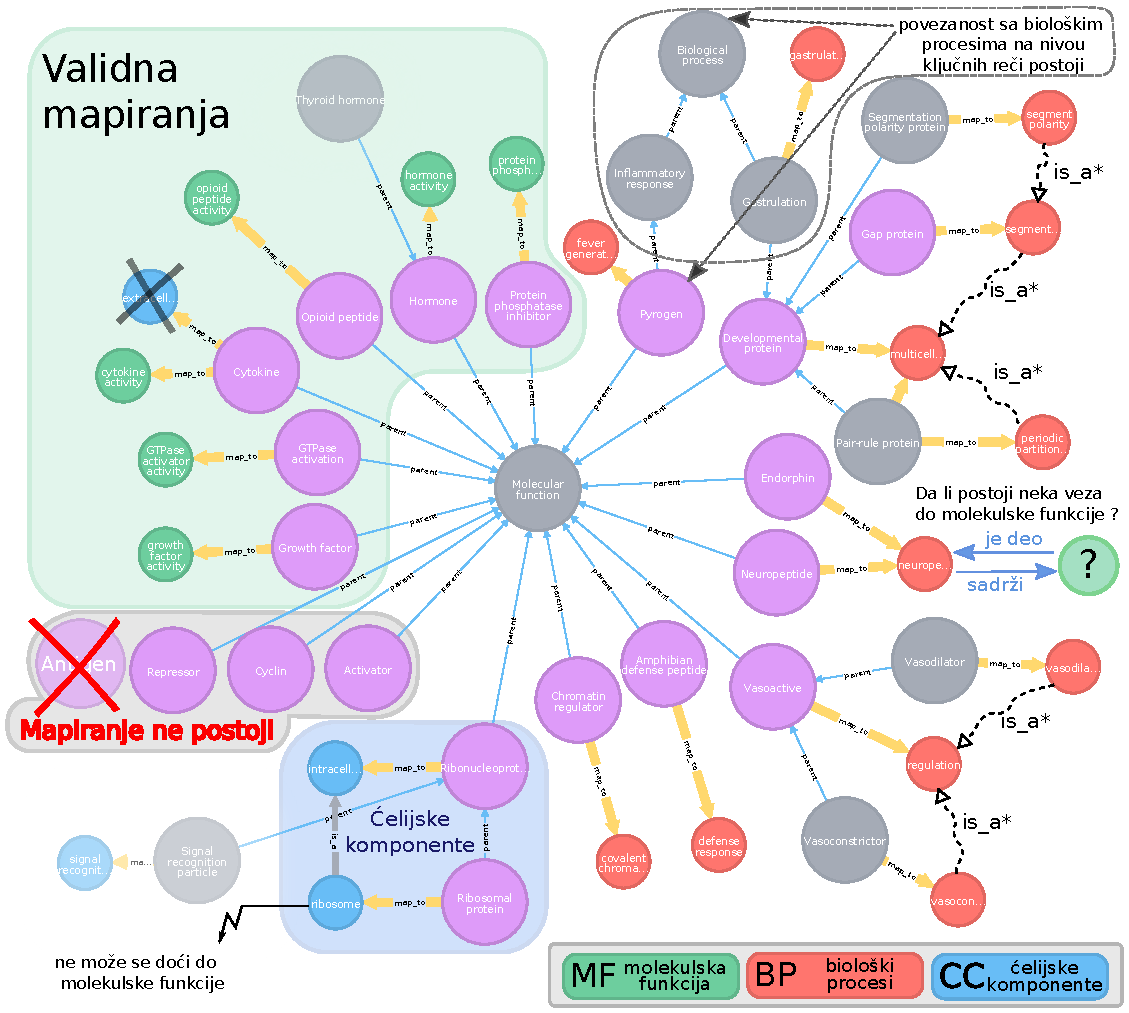
\includegraphics[scale=1]{Figures/plots/kw_dis2go.pdf}
\decoRule
\caption {
  Mapiranje 20 najznačajnijih neuređenih MF ključnih reči \parencite{Xie2007} 
  na GO termine.
}
\label{fig:KWtop20dis}
\end{figure}

Za neke BP termine moguće je doći do molekulske funkcije praćenjem veza \keyword{je
deo} ili \keyword{sadrži}. Međutim od 8 bioloških procesa prikazanih na Slici
\ref{fig:KWtop20dis} ovo je moguće samo za Neuropeptid.
\keyword{Cypher} upitom:
\begin{verbatim}
MATCH p=(:Keyword {name:"Neuropeptide"})--(:GOTerm)<-[*0..]-(:GOTerm)<--(:Protein)
RETURN p
\end{verbatim}
pronašli smo mapiranje na MF \textit{neuropeptide receptor activity}
predstavljeno Slikom \ref{fig:neuropeptide}.  Nažalost, uočava se da MF termini
i ključna reč Neuropeptid sadrže svega 5 zajedničkih proteina. Ovo je očekivano
s obzirom da pronađeni MF termin predstavlja proteine koji se vezuju za
neuropeptide.

Mi pretpostavljamo da je neuspešnost mapiranja posledica veze \keyword{je deo} koja ne
podrazumeva kompoziciju (\keyword{sadrži}) već samo agregaciju. Relacija
agregacije podrazumeva da molekulska funkcija postoji nezavisno od biološkog
procesa za razliku od relacije kompozicije. Kod pomenutih osam BP termina i njihovih
specijalizacija ne javlja se veza \keyword{sadrži}.
Dakle automatsko poređenje moguće je samo za šest od 20 originalnih neuređenih MF 
ključnih reči. Za uređene ključne reči postoji više direktnih mapiranja ali njih
ovde nećemo navoditi.

Konačni metod koji koristimo da dopunimo gore pomenuto mapiranje je
poluautomatski. Ključne reči od intersa ili njihove delove slažemo u 
regularan izraz oblika:
\begin{verbatim}
  # words je lista ključnih reči ili njihovih delova
  # re.I znači izjednačavanje malih i velikih slova
  expresion = re.compile( f"({'|'.join(words)})[^ ,.)]*", re.I )
\end{verbatim}
Konstruisani regularan izraz iskorišćen je na sledeći način. Prvo se pretražuje
da li ime GO termina sadrži neku reč iz regularnog izraza. Ako ne, pretraga se
proširuje na  sinonime GO termina. Ako ni tu nije pronađena, pretraživanje se
proširuje na definiciju termina. Rezultat su tri vrste relacije opadajuće
pouzdanosti (ime, sinonim, definicija). Zajedno sa originalnim direktnim
mapiranjima i pažljivom ručnom analizom moguće je dopuniti mapiranje i izvesti
poređenje rezultata. Pri analizi rezultata neophodno je uzeti u obzir
standardne definicije GO termina i sinonima navedenih u Potpoglavlju \ref{MF}.

Pomenuto mapiranje vršimo nad statistički značajnim (ne)uređenim MF
terminima.  U slučaju da se ključna reč ne pronađe pretraga se može izvesti za
deo imena ključne reči, međutim ovaj pristup može dovesti do netačnog
mapiranja. Sasvim je moguće da ključna reč nije pronađena jer odgovarajući MF
termini nisu statistički značajni što se mora zasebno proveriti. Smatramo da je
opisan metod uspešan zbog konzervativnosti fraza koje tražimo kao i informacije
o sinonimima koje GO termini sadrže.

Ključne reči često imaju karakter '-' koju GO termini izbegavaju. Zamena blanko
oznakom je neophodna za pretraživanje imena, ali ne i za sinonime koji često
sadrže '-' karakter. 


\begin{figure}[th]
\centering
\hspace*{-1.0cm} 
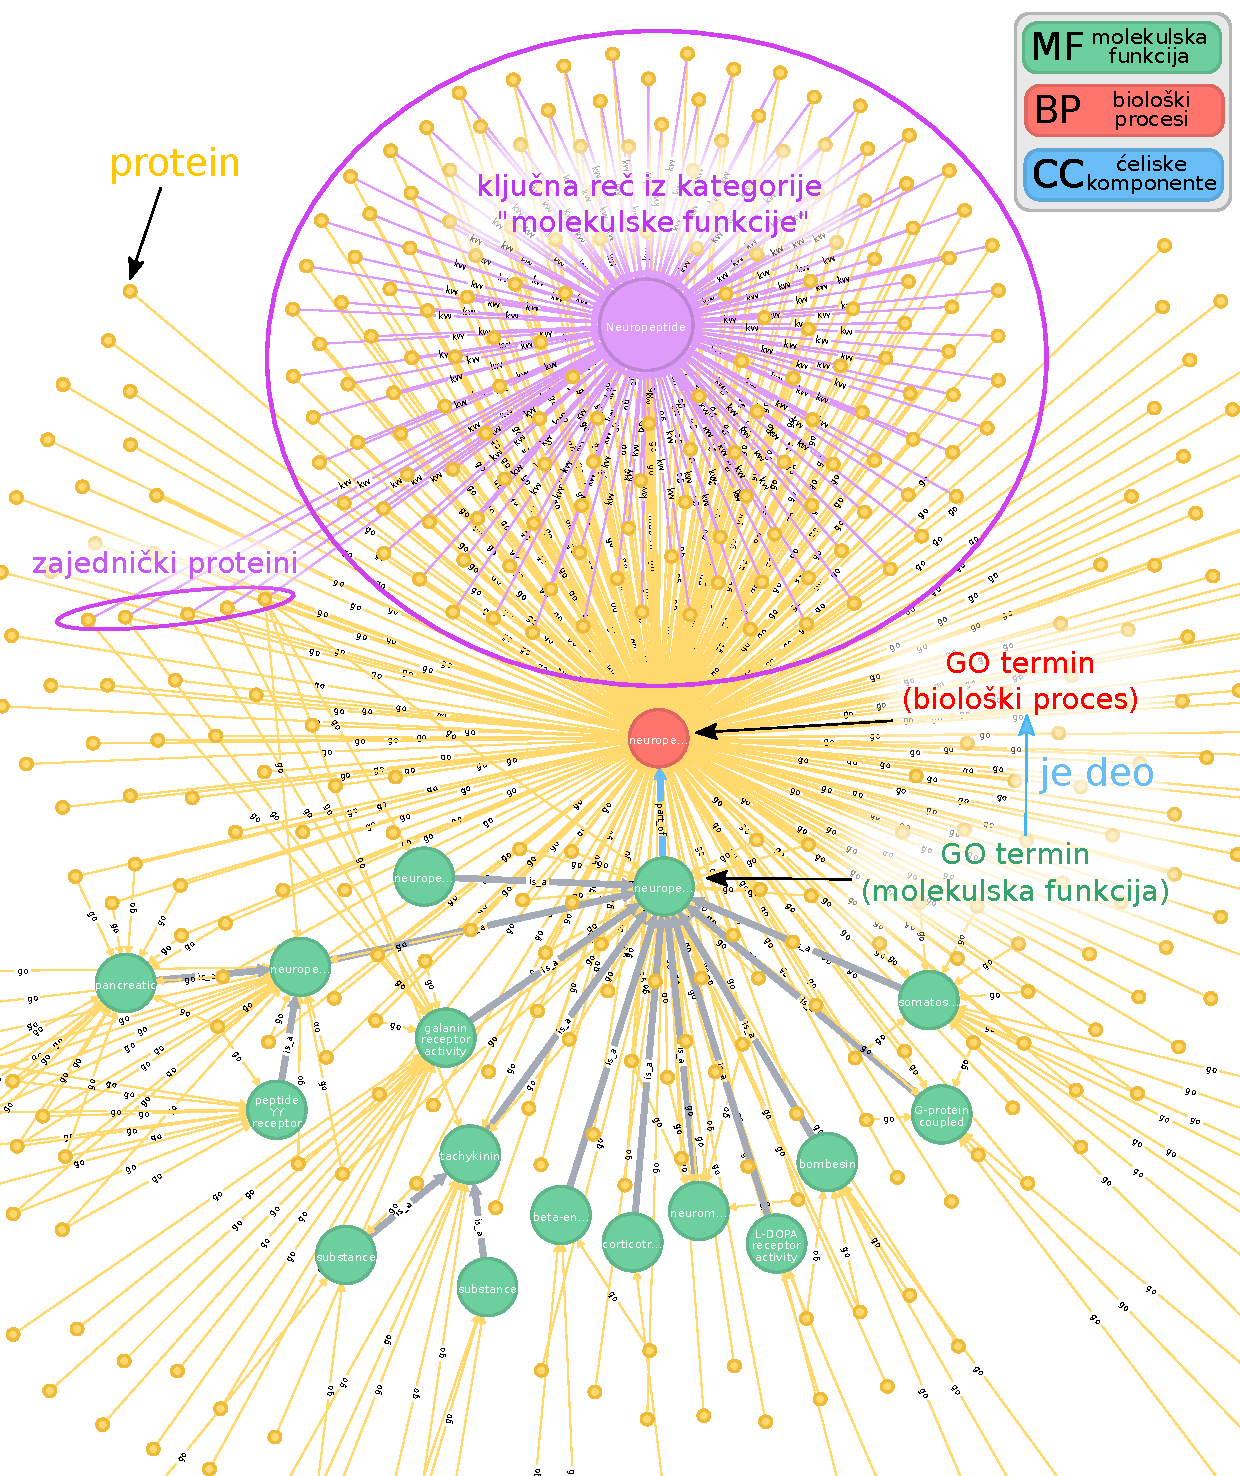
\includegraphics[scale=0.8]{Figures/plots/Neuropeptide2go.pdf}
\decoRule
\caption {
  Mapiranje ključne reči \keyword{Neuropeptid} na MF termine preko veze ''je deo''.
  Ovako postignuto mapiranje rezultuje malim brojem zajedničkih proteina.
}
\label{fig:neuropeptide}
\end{figure}
